%%
% The BIThesis Template for Graduate Thesis
%
% Copyright 2020-2023 Yang Yating, BITNP
%
% This work may be distributed and/or modified under the
% conditions of the LaTeX Project Public License, either version 1.3
% of this license or (at your option) any later version.
% The latest version of this license is in
%   http://www.latex-project.org/lppl.txt
% and version 1.3 or later is part of all distributions of LaTeX
% version 2005/12/01 or later.
%
% This work has the LPPL maintenance status `maintained'.
%
% The Current Maintainer of this work is Feng Kaiyu.
%
% Compile with: xelatex -> biber -> xelatex -> xelatex

\chapter{Connecting Action Semantics and Human Motion using Fuzzy Qualitative Kinematics}

Human motion understanding is fundamental to various applications in computer graphics, human-robot interactions, digital environments, and entertainment. Existing approaches predominantly rely on modeling motion with quantitative or qualitative kinematic facts. However, they often struggle to establish a robust connection between motion and corresponding action semantics...

\section{Introduction}
Human motion understanding is integral to numerous applications, including human-robot interaction, automated computer animations, social humanoid in augmented/virtual reality, intelligent non-playing characters (NPCs) in video games, physical fitness, sport analysis, and digital film production \cite{fg-t2m, act-recog, assist-walk}. The fundamental challenge lies in establishing a meaningful connection between the raw motion space and action semantic space ...
.

\section{Related Work}
\subsection{Human Motion Representation} 
An accurate representation of human motion is critical for generating realistic motion sequences \cite{motion-synthesis-survey}. Conventional motion is typically represented as a sequence of static pose representations characterized by joint...

\begin{figure*}[!t]
	\centering
	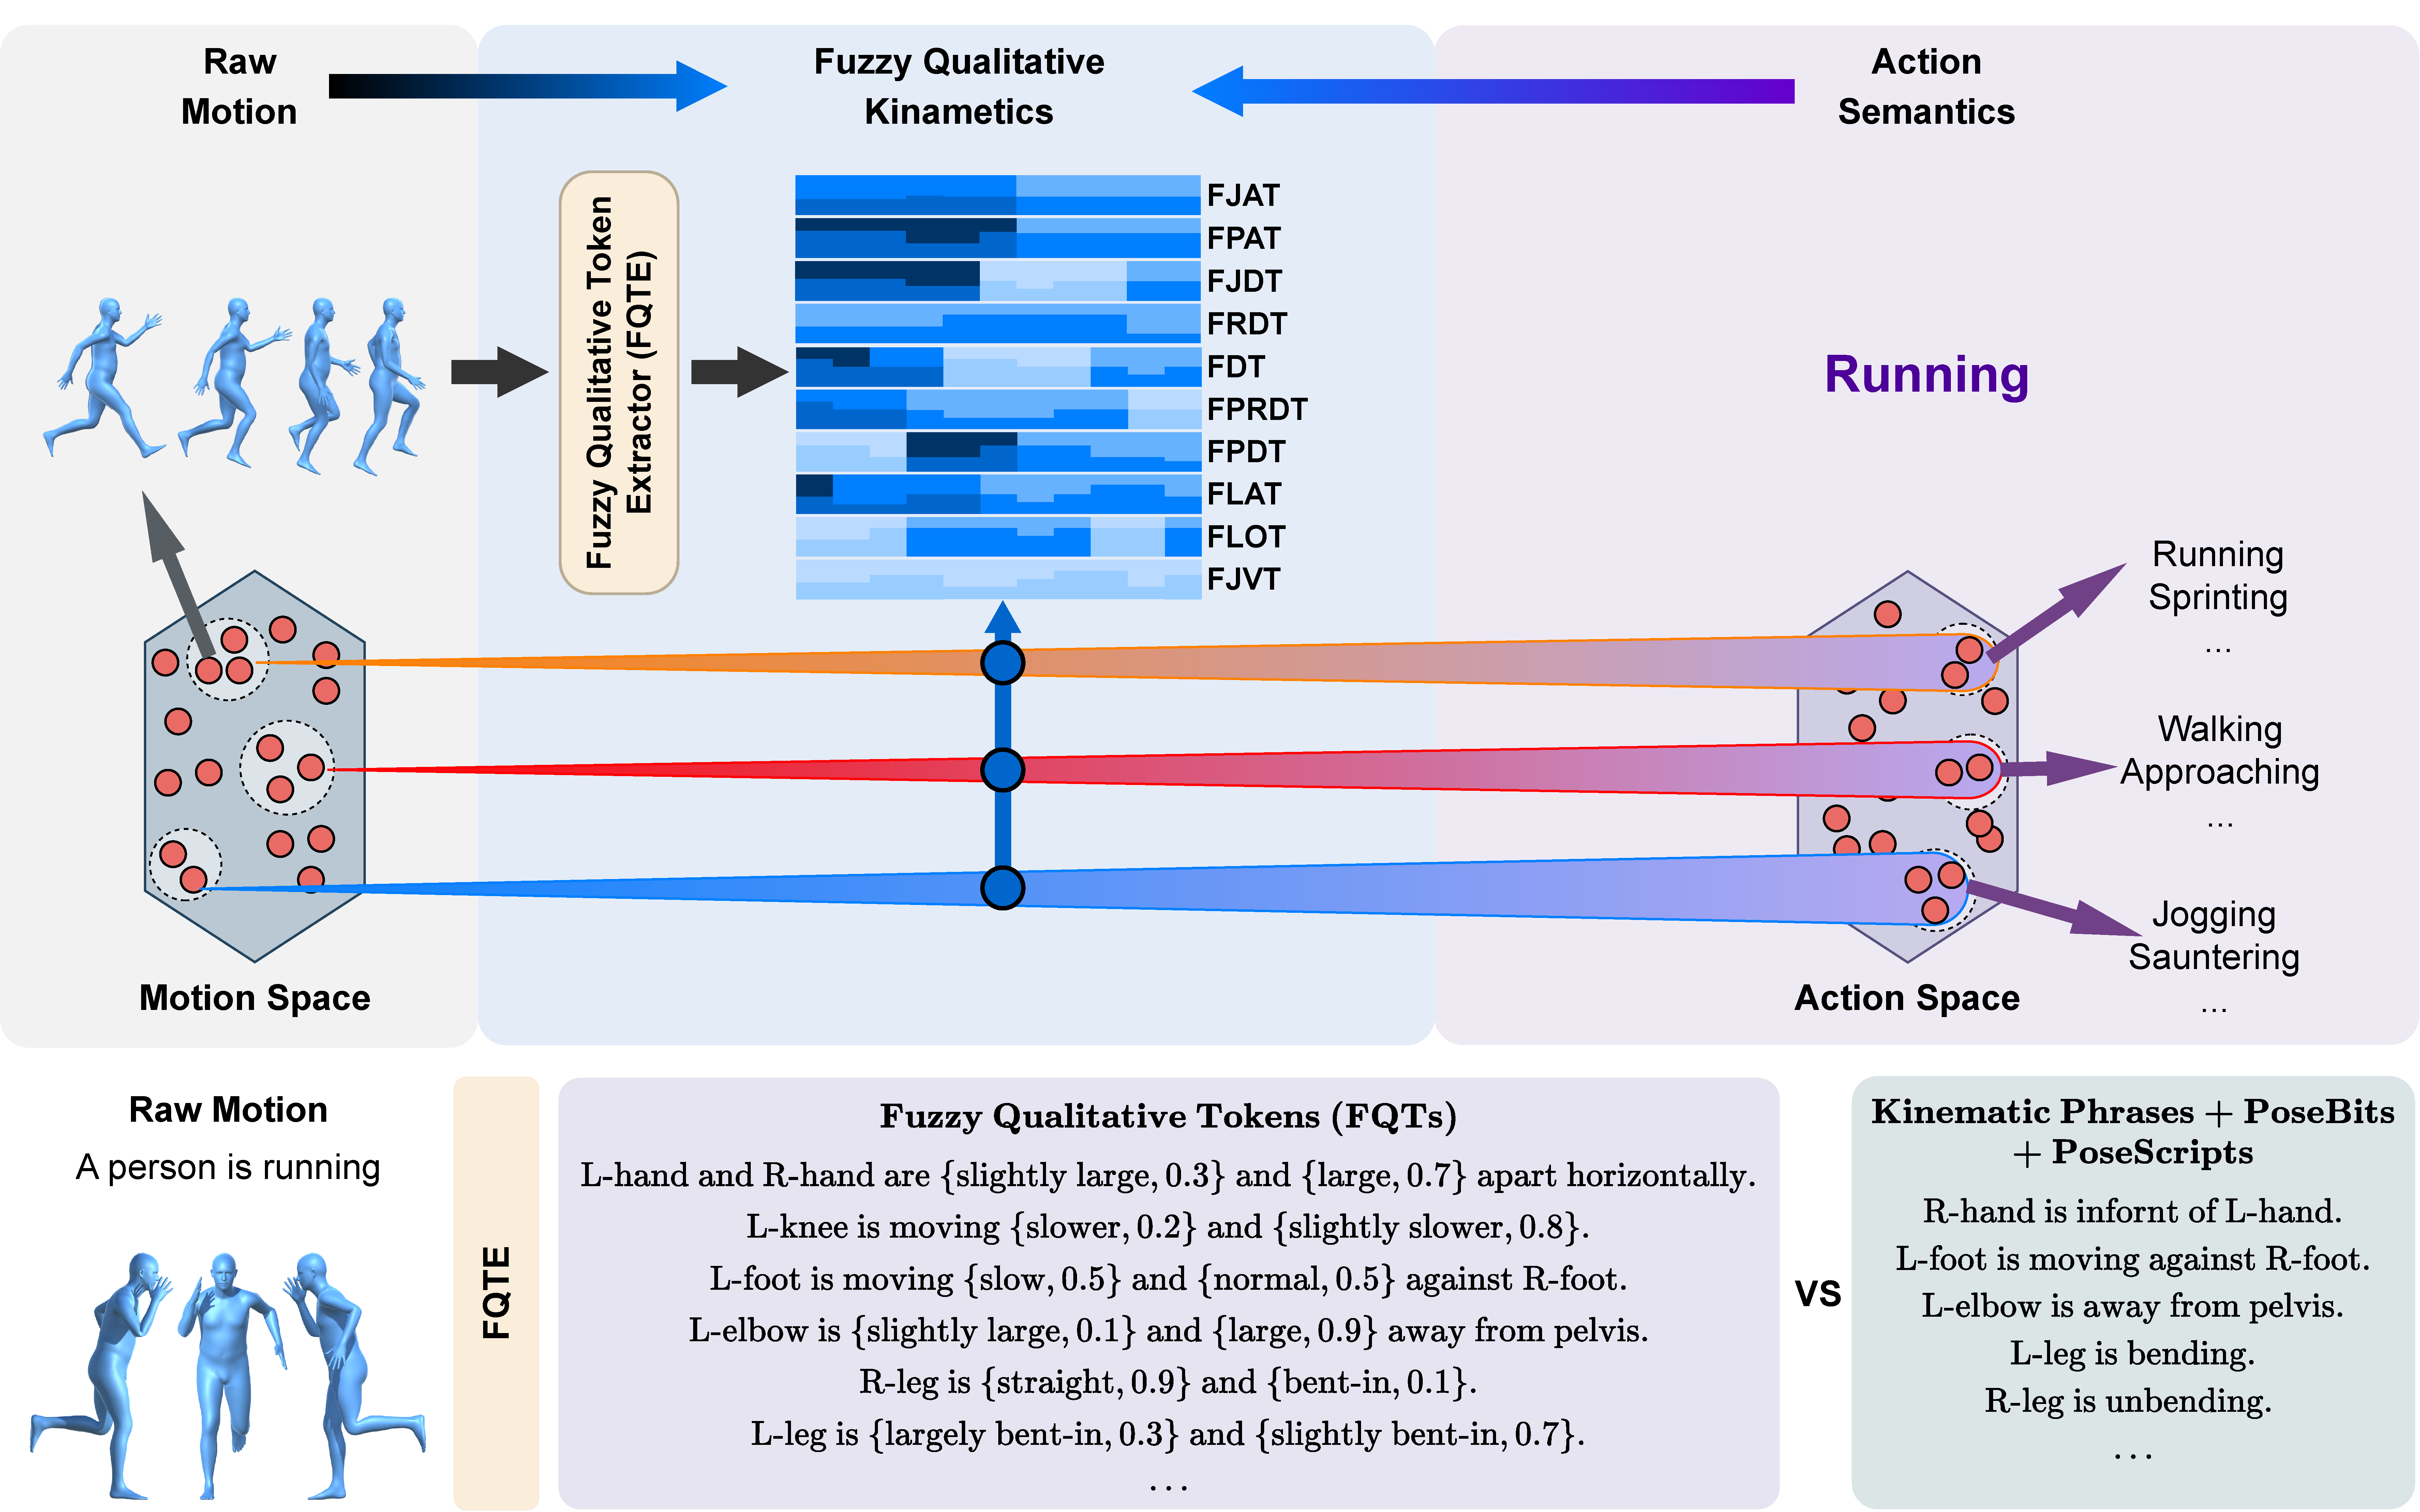
\includegraphics[width=1\textwidth]{figures/chapter3/fig_semantic_gap}
	\caption{(Top) Illustrates the gap between two motion modalities, i.e., raw motion and action descriptions. Understanding human motion requires modeling a complex many-to-many mapping function between motion and action spaces. Fuzzy Qualitative Tokens (FQTs) are presented as an intermediate representation to bridge the gap (bottom) comparison of boolean kinematic facts used by previous studies \cite{kinematic-phrases, pose_bits, pose_script} with our FQTs. FQTs provide expressive pose geometry and rich semantic information.}
	\label{fig_gap}
\end{figure*}




\section{Method}
\noindent
Effective mapping between the action and motion spaces is key to the success of any task involving motion. Fig. \ref{fig_gap} visually demonstrates the semantic gap between these two ...

\subsection{Quantized Fuzzy Membership Function}
\noindent
The standard fuzzy membership function assigns membership scores to crisp input values. However, the conventional real-value membership scale is computationally expensive. To address this issue, we introduce a quantized fuzzy membership function that strikes a balance between representational accuracy and computational complexity, as shown in Fig. \ref{fig_fuzzy}. This quantized fuzzy function extends the standard membership function by translating the real-valued membership scale into a quantized scale. The standard and quantized membership functions represented by the four-tuple $\left[ a, b, c, d \right] $ are defined by eq \eqref{eq_smem} and \eqref{eq_qmem}, respectively.
\begin{equation}
	\label{eq_smem}
	\mu(x) = 	
	\begin{cases}
		0 & \text{if } x \leq a \\
		(x-a)/(b-a), & \text{if } a \leq x \leq b \\
		1, & \text{if } b \leq x \leq c \\
		(d-x)/(d-c), & \text{if } c \leq x \leq d \\
		0, & \text{if } d \leq x
	\end{cases}
\end{equation}
\begin{equation}
	\label{eq_qmem}
	\dot{\mu}(x) = \lfloor \mu(x) \times \mu_{ql} \rfloor /\mu_{ql}
\end{equation}

Where $\mu(.)$ and $\dot{\mu}(.)$ are the standard and quantized membership functions, respectively. The $x$ denotes the crisp value, with $\mu_{ql}$ referring to the number of quantization levels. 



\begin{figure}
	\centering
	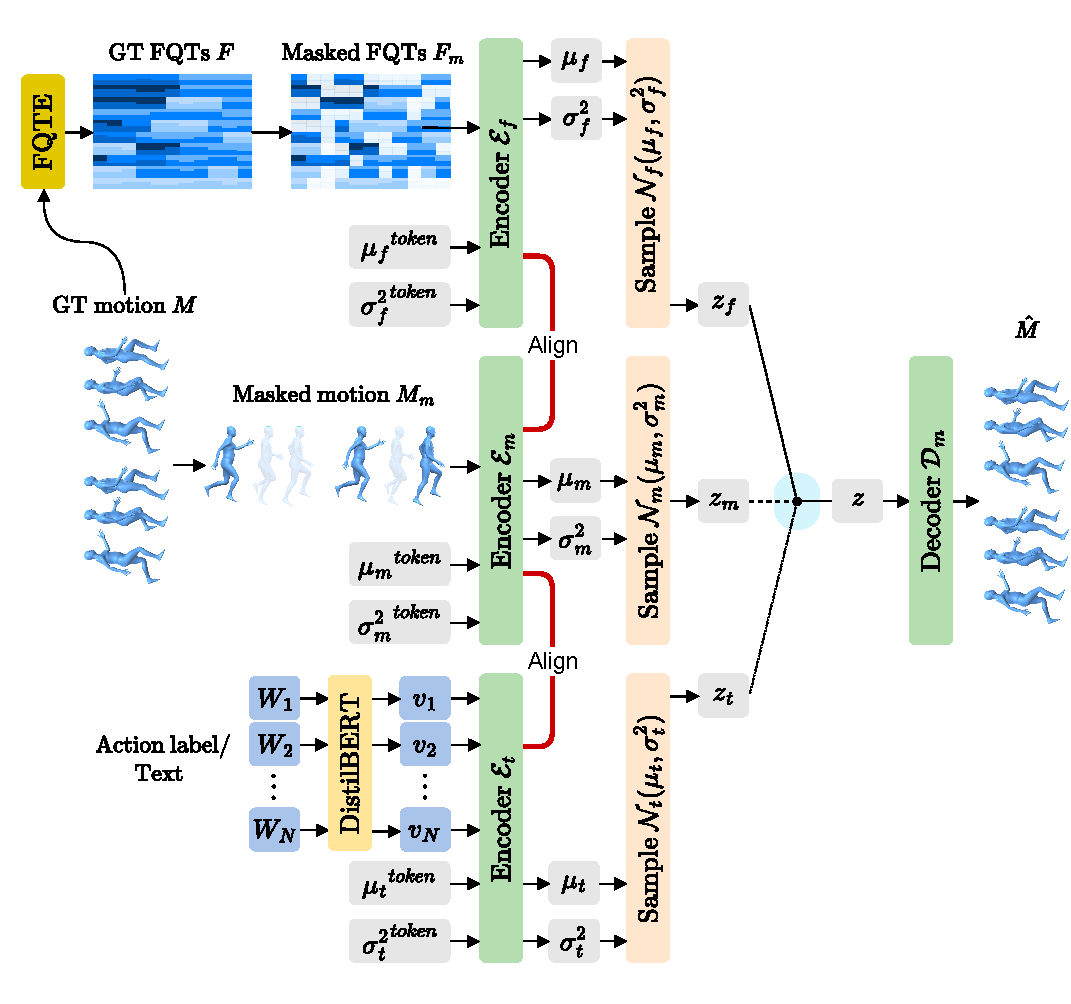
\includegraphics[width=1\textwidth]{figures/chapter3/fig_model}
	\caption{Method overview: During training, we encode FQTs, motion and text through their respective transformer encoders, together with modal-specific learnable distribution tokens. Each encoder outputs Gaussian distribution parameters, subject to KL losses, from which a latent vector $z$ is sampled. The decoder uses the sampled variable to interpolate, predict, and generate a motion sequence.}
	\label{fig_model}
\end{figure}

